%\documentclass[12pt]{jarticle}



\chapter{はじめに}
\label{chap:introduction}
\pagenumbering{arabic}


%序論の目安としては1枚半ぐらい.
%英語発表者は,最終予稿の「はじめに」の英訳などを載せてもいいかも.



\section{背景と目的}
近年、地球温暖化等の影響で台風や異常気象など天候の変化が激しい\cite{earth}。これらの天候変化は船舶の運航状況に支障をきたす。運航状況への支障として、船舶利用者が利用したいときに運航できない場合や貨物を運ぶ際に予定通りに運ぶことができないということがある。なかでも、旅客船に考えられる被害として、突然の欠航により船舶利用者の予定に支障が出る可能性がある。それにより経済的損失が発生する問題があると考えられる。船舶の運航を決定づける権限を持つのは船長であり、自身の経験に基づき気象通報、水路通報その他の航海に必要な情報を参考にすることで運航当日に決定している\cite{stan}。筆者は当日にしか公表されない船舶の運航状況を数日前に予測することで観光客や船舶の利用者のスケジュール組立ての一助を目指す。
関連研究として沿岸波浪および、船体運動データを用いたシミュレーションによる新たな欠航判断基準を提供するものがある\cite{Related-Research1}。この研究では船体運動などのデータが必要不可欠であり、そのデータを取得するのは簡単ではないため、データ取得の容易な気象状況の値、あるいは予報図から船舶の欠航を予測したいと考えた。本研究では機械学習を用い、過去の欠航データ、気象データを活用し数日先までの欠航を予測することを目的とし実験を行う。

\section{関連研究}
\subsection{欠航判断においての研究事例}
笹\cite{Related-Research1}らは運航判断において航海中の波浪の角度、周期が反映された船体運動にて評価すべきと考えている。そのため台風接近時のフェリーを検証対象とし船体運動データを観測した。また沿岸波浪(ナウファス)\cite{nowphas}と観測データをもとに船体運動のシミュレーションを実施し、検証した。これらの結果からフェリー欠航の新たな判断基準を提案するための基礎的研究を行った。
\\ 問題点として船体運動の縦揺れの再現結果が実測値よりも過小評価していることが挙げられる。シミュレーションの再現結果では船体の実際の有義振幅が6.76°であるのに対し計算結果では2.61°と半分以下の値が出力されている。有義振幅とは、ある地点で観測された連続値のデータの大きい方から全体の$1/3$の個数を平均して計算した振幅となる。また、シミュレーションに使用するデータが船体を観測して得られるデータのため、様々なフェリー航路への応用が難しく、データの取得が容易でない。そのため本研究では、データ取得が比較的容易である天気予報webサイトなwindy\cite{windy}や運航状況を確認できる安栄観光\cite{anei}などのサイトを使用しデータを活用して欠航の予測を行う。

\subsection{降雨レーダー画像を入力とした機械学習での予測においての研究事例}
Jason\cite{Related-Research2}らはディープラーニング(CNN)をモデルとして入力に降雨レーダー画像を使用し、出力に数時間先の降雨レーダー画像を生成するCNNを構築し、降雨量を予測することを目的に研究を行った。これをナウキャスティングという。降雨レーダー画像はMRMS\cite{MRMA}と呼ばれる$1km\times1km$の解像度で2分毎に得られるシステムを使用する。MRMSから得られるの2017年7月から2019年7月の期間のデータを使用する。画像の教師ラベルを降雨量の閾値0,0.1,1.0,2.5以上の4つの離散範囲に量子化する。2018年分のデータをトレーニングし、2017年と2019年をテストデータとして検証を行った。
\\ 図\ref{R_r_r}は左が入力画像で中央が1時間先の降雨予測、右が1時間先の実際の降雨となっている。
より具体的なモデルの構築内容は図\ref{rainfull_m}となっており、CNNのU-Netを使用している。
\begin{figure}[H]
 \centering
 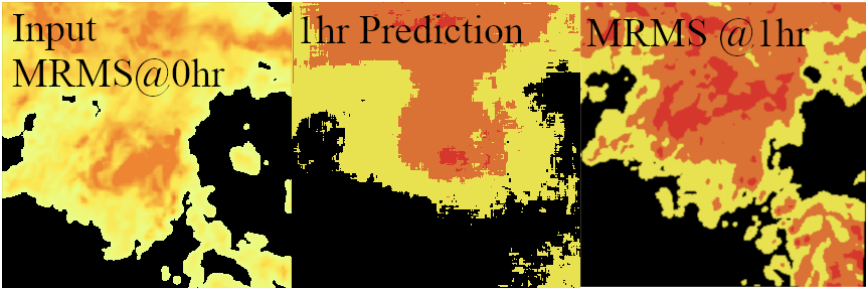
\includegraphics[keepaspectratio, scale=0.5]{fig/chapter1/Related_research_rainfall.png}
 \caption{1時間後先の降雨予測比較\cite{Related-Research2}}
 \label{R_r_r}
\end{figure}

\begin{figure}[H]
 \centering
 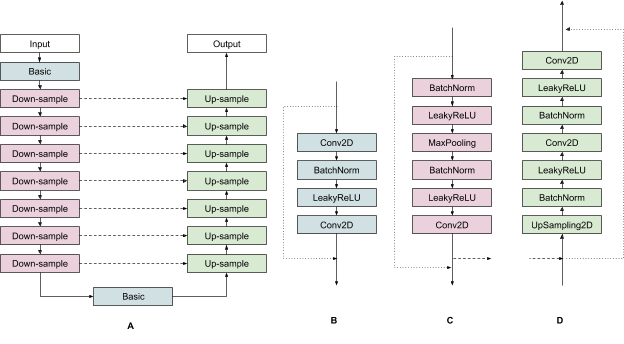
\includegraphics[keepaspectratio, scale=0.4]{fig/chapter1/rainfull_model.png}
 \caption{CNNモデルの詳細\cite{rainfull}}
 \label{rainfull_m}
\end{figure}
Jasonらの研究によるとこのCNNモデルを使用した1時間先の予測結果は既存のモデルoptical flow\cite{optical-flow}、persistence\cite{persistence}、HRRR nowcasting\cite{HRRR}と比較して精度が良くなるという研究結果がある。しかし、5時間先の予測の比較ではHRRRが良いという結果となった。\\
 結論としては 1 時間先という短時間予測においては CNN による画像から画像への予測変換モデルの有効性を示している。降水量の複雑な物理学をモデル化し、シミュレーションの時間がかかる手法をデータを入出力問題として扱うことで、1時間先の予測は良好であることを示している。しかしながら、HRRRと機械学習の両方のアプローチの組み合わせが問題として残る。\\
 Jasonらの研究を踏まえて降雨レーダー画像を使用した機械学習の問題ではCNNモデルがより良い精度を獲得できることがわかる。また、CNNを使用する理由の一つとして画像のデータの追加、交換が容易であることとしている。\\
 本研究では天候データである画像は地球の任意の場所で取得できるということもあり、特定の地域だけでなく任意の航路の欠航予測を行うこともできる拡張性に着目し、採用する。また、降雨レーダー画像と本研究で使用するデータセットの画像、図\ref{wind_data}、図\ref{wave_data}とは風、波と降雨のようにレイヤーが異なるだけなのでCNNモデルが有効だと考える。本研究の入力データは画像だが出力データは運航、欠航の2値分類のため出力結果を2値のクラス分類にする必要がある。
%そのため本研究でも画像入力の場合にCNNモデルを採用する。

%Jasonらの研究によってCNNが降雨レーダー画像に対して有効であると示されたために、本研究では天気予報の画像を入力データとして使用するため、学習モデルとしてCNNを用いる

%新しく「1.3 本研究の位置づけ」ぐらいの節を追加しよう。中身は、(1) 二値分類タスクとしての特徴(例えばレビュー分析のネガポジ判定と何が違うのか)、(2)天候予測との違い、(3)画像データや数値データとしての特徴(例えばImageNetとの違いは)、(4)時系列データとしての特徴、あたりを盛り込めるとベストです。(全部である必要はありません。少なくとも重要なポイントは示そう)
\section{本研究の位置づけ}
本研究は船舶の運航状況を欠航か運航か分類する二値分類タスクである。使用するデータとしては運航か欠航であるかの二値の教師データ、そこに付随する特徴量として数値データ(風速や波の高さ等)または画像データの2種類がある。これらの2種類のデータを分けて学習モデルに学習させ違いを比較することで、本研究の船舶での予測を行う際の最適なデータを検討する一助を目指し、さらに数値だけでの予測よりも精度向上を望めないか検討する。また、数日先までの予測を数値を使用した予測と画像を使用した予測を行った場合との違いを比較、考察を行い、数値と画像との精度評価を実施する。%どのようなデータが誤った予測しやすいのか明らかにしていく。

%画像を使用した機械学習としてImageNetが存在しているがImageNetでは様々な自然画像に対してそれぞれ1つずつラベルがついており、


%二値分類タスクでは他にレビュー分析のネガポジ判定がある。本研究では数値予測の他に画像での予測を行う、これは学習モデルに入力する情報が数値よりも画像の方がより多くの情報を持つのではないかと考えた結果である。

%\newpage

\section{論文の構成}
本論文は、以下の通りに構成されている。
\\
\\
\large{\textbf{第1章 はじめに}}\\
\ \ \ \ 本研究の背景と目的について述べる。\\
\large{\textbf{第2章 基礎概念}}\\
\ \ \ \ 提案手法に関することについて述べる。\\
\large{\textbf{第3章 提案手法}}\\
\ \ \ \ 機械学習の実装とデータ作成に関することについて述べる。\\
\large{\textbf{第4章 実験}}\\
\ \ \ \ 実験と考察について述べる。\\
\large{\textbf{第5章 今後の課題}}\\
\ \ \ \ 提案手法と検証に関する今後の課題を述べる。\\
\normalsize{}


%\section{Introduction}
